% EVALUATION. Numbers ONLY via \R... macros from generated/numbers.tex.
\subsection{Setup}
\textbf{Task families.} Each family has \RNPerFamily instances, split once by a seeded shuffle into \RNDev development
and \RNTest test instances, with test hashes locked before any test run. \emph{Facts}: HotpotQA distractor questions
(validation split)~\citep{hotpotqa2018}; each instance carries its native paragraphs plus extra distractors drawn from other
questions (\RNumDocs documents, \RFullTokFacts tokens on average over all instances), two worked examples, and asks for a short answer.
\emph{Tool}: a call from the Berkeley Function Calling Leaderboard (BFCL v3) of the Gorilla project~\citep{gorilla2023} (simple and multiple categories); the
correct function or functions are mixed into a \RNumTools-tool catalog (\RFullTokTool tokens), and success is an
AST-level match of the emitted call. \emph{History}: \RNumSessions synthetic chat sessions (\RFullTokHistory tokens)
in which one user attribute is set and later updated, a knowledge-update setting also probed by
LongMemEval~\citep{longmemeval2024}; the agent must report the latest value, and in half of the
instances a note restates the \emph{stale} value. Success checks are deterministic.

\textbf{Models.} Qwen3-4B-Instruct-2507 (Ollama tag \texttt{qwen3:4b-instruct}, a non-thinking release) is the main
model and the profiling source; Qwen3-8B (tag \texttt{qwen3:8b}, the earlier hybrid-thinking release, run with thinking
disabled) is the transfer target, so transfer spans both model size and post-training release. Both are the default
4-bit Ollama builds (model digests in the run manifests) and run locally with greedy decoding, a fixed seed, a
\RNumCtx-token window and at most \RNumPredict output tokens.

\textbf{Policies.} B0 full context (no budget); B1 truncate oldest; B2 embedding relevance (nomic-embed-text cosine to
the goal, fill in descending order); B3 LLMLingua-2~\citep{llmlingua2_2024} compressing all optional context to the
remaining budget; B4 a PACMS-style facility-location coverage selector~\citep{pacms2026} (our re-implementation); B5 fixed
type tiers; OURS-A, the MCV compiler without interaction terms; OURS, with them. All policies keep the mandatory blocks
and share the renderer.

\textbf{Protocol.} Profiles use the first \RNProfFour development instances (4B, with \RNLobo leave-one-block-out samples
each) and \RNProfEight instances (8B, type level). Budgets are 1k, 2k, 4k and 8k tokens. The primary metric is the area
under the success--budget curve (AUBC), normalized over log-budget, per instance. The main grid evaluates B0, B2, B4,
OURS-A and OURS on the first \RNMain test instances per family; the weaker baselines B1, B3, B5 (well below B2 in dev
pilots) use the first \RNWeak. Following the pre-registration, H1 compares OURS with the best of B1--B5 per family; H1b
tests, at 8k, that OURS uses fewer tokens than B0 and the best baseline with success non-inferior to B0 (margin
\RMargin); H2 compares OURS with OURS-A pooled; H3 tests transfer. Intervals are paired percentile bootstraps
(\RNBoot resamples); p-values are Wilcoxon signed-rank for H1 and H2 and a one-sided paired bootstrap for H1b (the plan fixed the CI rule but named no test; recorded as a deviation); H1, H1b and H2
form one Holm family. All \RMainEpisodes main episodes completed. Block costs are summed in the model's tokenizer;
rendered prompts exceeded the budget in \ROverBudgetMain of \RBudgetedMain budgeted main-study episodes, by at most
\RMaxOvershoot tokens, because tokens merge at block boundaries.

\begin{table}[t]\centering\small
\caption{Test results on Qwen3-4B-Instruct: AUBC (mean, 95\% paired-bootstrap CI) and success at the 1k and 8k budgets.
B1, B3 and B5 use the first \RNWeak instances per family, the others \RNMain. B0 ignores the budget, so its 1k and 8k
entries are the same full-context run.}\label{tab:main}
\setlength{\tabcolsep}{2.6pt}
\fitwidth{%
\begin{tabular}{@{}l ccc ccc ccc@{}}\toprule
& \multicolumn{3}{c}{Facts (HotpotQA)} & \multicolumn{3}{c}{History (synthetic)} & \multicolumn{3}{c}{Tool (BFCL)}\\
\cmidrule(lr){2-4}\cmidrule(lr){5-7}\cmidrule(lr){8-10}
Policy & AUBC & @1k & @8k & AUBC & @1k & @8k & AUBC & @1k & @8k\\\midrule
B0 full & \RAubcFactsFull {\scriptsize[\RAubcFactsFullLo, \RAubcFactsFullHi]} & \RSucFullFacts & \RSucFullFacts & \RAubcHistoryFull {\scriptsize[\RAubcHistoryFullLo, \RAubcHistoryFullHi]} & \RSucFullHistory & \RSucFullHistory & \RAubcToolFull {\scriptsize[\RAubcToolFullLo, \RAubcToolFullHi]} & \RSucFullTool & \RSucFullTool\\
B1 truncate oldest & \RAubcFactsTrunc {\scriptsize[\RAubcFactsTruncLo, \RAubcFactsTruncHi]} & \RSucFactsTruncOne & \RSucFactsTruncEight & \RAubcHistoryTrunc {\scriptsize[\RAubcHistoryTruncLo, \RAubcHistoryTruncHi]} & \RSucHistoryTruncOne & \RSucHistoryTruncEight & \RAubcToolTrunc {\scriptsize[\RAubcToolTruncLo, \RAubcToolTruncHi]} & \RSucToolTruncOne & \RSucToolTruncEight\\
B2 relevance & \RAubcFactsRel {\scriptsize[\RAubcFactsRelLo, \RAubcFactsRelHi]} & \RSucFactsRelOne & \RSucFactsRelEight & \RAubcHistoryRel {\scriptsize[\RAubcHistoryRelLo, \RAubcHistoryRelHi]} & \RSucHistoryRelOne & \RSucHistoryRelEight & \RAubcToolRel {\scriptsize[\RAubcToolRelLo, \RAubcToolRelHi]} & \RSucToolRelOne & \RSucToolRelEight\\
B3 LLMLingua-2 & \RAubcFactsLingua {\scriptsize[\RAubcFactsLinguaLo, \RAubcFactsLinguaHi]} & \RSucFactsLinguaOne & \RSucFactsLinguaEight & \RAubcHistoryLingua {\scriptsize[\RAubcHistoryLinguaLo, \RAubcHistoryLinguaHi]} & \RSucHistoryLinguaOne & \RSucHistoryLinguaEight & \RAubcToolLingua {\scriptsize[\RAubcToolLinguaLo, \RAubcToolLinguaHi]} & \RSucToolLinguaOne & \RSucToolLinguaEight\\
B4 coverage (PACMS-style) & \RAubcFactsCov {\scriptsize[\RAubcFactsCovLo, \RAubcFactsCovHi]} & \RSucFactsCovOne & \RSucFactsCovEight & \RAubcHistoryCov {\scriptsize[\RAubcHistoryCovLo, \RAubcHistoryCovHi]} & \RSucHistoryCovOne & \RSucHistoryCovEight & \RAubcToolCov {\scriptsize[\RAubcToolCovLo, \RAubcToolCovHi]} & \RSucToolCovOne & \RSucToolCovEight\\
B5 type tiers & \RAubcFactsTier {\scriptsize[\RAubcFactsTierLo, \RAubcFactsTierHi]} & \RSucFactsTierOne & \RSucFactsTierEight & \RAubcHistoryTier {\scriptsize[\RAubcHistoryTierLo, \RAubcHistoryTierHi]} & \RSucHistoryTierOne & \RSucHistoryTierEight & \RAubcToolTier {\scriptsize[\RAubcToolTierLo, \RAubcToolTierHi]} & \RSucToolTierOne & \RSucToolTierEight\\
OURS-A (MCV additive) & \RAubcFactsAdditive {\scriptsize[\RAubcFactsAdditiveLo, \RAubcFactsAdditiveHi]} & \RSucFactsAdditiveOne & \RSucFactsAdditiveEight & \RAubcHistoryAdditive {\scriptsize[\RAubcHistoryAdditiveLo, \RAubcHistoryAdditiveHi]} & \RSucHistoryAdditiveOne & \RSucHistoryAdditiveEight & \RAubcToolAdditive {\scriptsize[\RAubcToolAdditiveLo, \RAubcToolAdditiveHi]} & \RSucToolAdditiveOne & \RSucToolAdditiveEight\\
OURS (MCV + interactions) & \RAubcFactsOurs {\scriptsize[\RAubcFactsOursLo, \RAubcFactsOursHi]} & \RSucFactsOursOne & \RSucFactsOursEight & \RAubcHistoryOurs {\scriptsize[\RAubcHistoryOursLo, \RAubcHistoryOursHi]} & \RSucHistoryOursOne & \RSucHistoryOursEight & \RAubcToolOurs {\scriptsize[\RAubcToolOursLo, \RAubcToolOursHi]} & \RSucToolOursOne & \RSucToolOursEight\\
\bottomrule\end{tabular}}
\end{table}

\begin{figure}[t]\centering
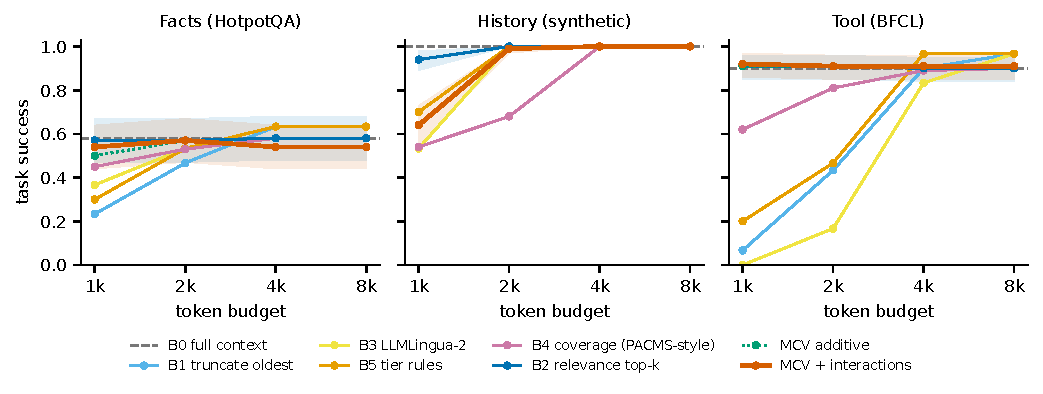
\includegraphics[width= 0.88\linewidth]{../figures/fig2_success_budget.pdf}
\caption{Success versus token budget on Qwen3-4B-Instruct (test). Bands: 95\% bootstrap CIs for B2 and OURS. The
dashed line is full context. MCV additive and MCV with interactions overlap almost everywhere.}\label{fig:curves}
\end{figure}

\begin{table}[t]\centering\small
\caption{Pre-registered hypotheses. Differences are paired (OURS minus comparator); H1 and H2 in AUBC, H1b and H3 in
success. $p$: Holm-adjusted over H1, H1b and H2 (two-sided Wilcoxon for H1 and H2, one-sided paired bootstrap for H1b);
H3 is decided by its CI against the margin \RMargin. Its interval is degenerate because transferred and native profiles
gave identical outcomes in every pair, so H3 passes without being informative (see the transfer results below).}\label{tab:hyp}
\setlength{\tabcolsep}{3pt}
\begin{tabular}{@{}llccl@{}}\toprule
Hyp. & Family & Difference [95\% CI] & $p$ & Outcome\\\midrule
H1 & Facts & \RHOneFactsDiff{} [\RHOneFactsLo, \RHOneFactsHi] & \RHOneFactsP & no gain\\
H1 & History & \RHOneHistoryDiff{} [\RHOneHistoryLo, \RHOneHistoryHi] & \RHOneHistoryP & worse\\
H1 & Tool & \RHOneToolDiff{} [\RHOneToolLo, \RHOneToolHi] & \RHOneToolP & no gain\\
H1b & Facts & \RHOnebFactsDiff{} [\RHOnebFactsLo, \RHOnebFactsHi] & \RHOnebFactsP & not shown\\
H1b & History & \RHOnebHistoryDiff{} [\RHOnebHistoryLo, \RHOnebHistoryHi] & \RHOnebHistoryP & non-inferior\\
H1b & Tool & \RHOnebToolDiff{} [\RHOnebToolLo, \RHOnebToolHi] & \RHOnebToolP & non-inferior\\
H2 & Pooled & \RHTwoPooledDiff{} [\RHTwoPooledLo, \RHTwoPooledHi] & \RHTwoPooledP & no effect\\
H3 & Pooled & \RTransferDiff{} [\RTransferLo, \RTransferHi] & -- & \RHThreeVerdict{}$^{*}$\\
\bottomrule\end{tabular}
\end{table}

\subsection{Main Result: H1 Is Not Supported}
Table~\ref{tab:hyp} summarizes all pre-registered tests. 
Table~\ref{tab:main} and Fig.~\ref{fig:curves} give the main comparison. Embedding relevance (B2) was the best baseline
in every family. OURS did not exceed it anywhere: the paired AUBC difference was \RHOneFactsDiff{}
[\RHOneFactsLo, \RHOneFactsHi] on facts and \RHOneToolDiff{} [\RHOneToolLo, \RHOneToolHi] on tool use, both
indistinguishable from zero, and \RHOneHistoryDiff{} [\RHOneHistoryLo, \RHOneHistoryHi] on history, a significant
\emph{loss} (Holm $p\RHOneHistoryPRel$). H1 required a significant gain in two families; it fails.

On tool use the MCV compiler beat the non-relevance baselines by wide margins at small budgets: at 1k it reached
\RSucToolOursOne success against \RSucToolLinguaOne for LLMLingua-2, \RSucToolTruncOne for truncation and
\RSucToolCovOne for coverage, because it spends the budget on the tool schemas ranked most valuable and often drops
examples. This advantage did not hold elsewhere: on history at 1k OURS (\RSucHistoryOursOne) trailed truncation
(\RSucHistoryTruncOne) and tiers (\RSucHistoryTierOne). Relevance ranking also concentrates the budget on goal-related blocks. Once a block's value is dominated by
whether it is about the goal, an embedding score already captures most of what the profile adds.

\textbf{Diagnosis of the history loss.} Almost all of the history gap arises at the 1k budget (at 2k and above both policies
are at or near ceiling). There, success depends almost only on whether the session containing the latest update
survives selection. OURS kept it in \RRecallOurs of plans and B2 in \RRecallRel; without that session OURS never
answered correctly (\RSucGivenNoGoldOurs). Two causes combine. The first is the block-value model. Trained on
leave-one-block-out deltas, its history coefficients (unstandardized; recency spans the unit interval, while goal similarity varies over a narrow range) weight recency (\RCoefRecency) and token length
(\RCoefLen) alongside embedding similarity (\RCoefSim), so it fills a small budget with the most recent sessions and
misses the update whenever it lies further back. The second is the profile itself, applied far from where it was
measured. The note's value (\RMcvHistoryNote) is a leave-one-type-out effect from the full context, where history already
supplies the answer, and the interaction term penalizes sending both. At 1k, OURS sent the note in \RNoteInOursOne of
plans, against \RNoteInRelOne for relevance, so when the update session was dropped no fallback remained. In an
exploratory check of the logs (not pre-registered), \ROursFailCurrentNote of the \ROursFailHistOne OURS failures at 1k
were instances whose note held the \emph{current} value, and policies that kept a current note but missed the update
session answered correctly in \RNoteRescueRate of \RNoteRescueN such episodes. A type value measured at full context is
therefore not a valid value at a small budget for types that are redundant only in the presence of others. The
leave-one-block-out signal is sparse: removing one of \RNumSessions sessions rarely changes the outcome, so the
regression learns weak correlates of value instead of value. An exploratory check on the development logs confirms this (not
pre-registered; five-fold cross-validation grouped by instance). Only \RCvNonzeroHistory of history-session deletions
changed the outcome (\RCvNonzeroFacts for documents, \RCvNonzeroTool for tool schemas). The cross-validated rank
correlation between predicted and observed deltas was \RCvModelHistory for the ridge model against \RCvSimHistory for
embedding similarity alone on history, \RCvModelFacts against \RCvSimFacts on facts, and \RCvModelTool for both on
tool use. The learned ranker was never better than its own similarity feature.

\subsection{Pruning: H1b Is Supported in Two of Three Families}
Because the compiler adds blocks only while they raise the predicted objective, it leaves budget unused at 8k
(Fig.~\ref{fig:composition}), whereas B2 fills the budget and so matches full context. On tool use OURS sent
\RTokOursTool tokens instead of \RTokFullTool (\RTokCutTool fewer) with success \RSucOursEightTool against
\RSucFullTool for full context (difference \RHOnebToolDiff, CI [\RHOnebToolLo, \RHOnebToolHi], Holm
$p\RHOnebToolPRel$). On history it sent \RTokCutHistory fewer tokens with identical success (\RSucOursEightHistory),
the saving coming from the examples, the note and a few low-value sessions. On facts it sent \RTokCutFacts fewer tokens,
but success fell from \RSucFullFacts to \RSucOursEightFacts and the CI [\RHOnebFactsLo, \RHOnebFactsHi] crosses the
margin, so non-inferiority is not shown there. Two families pass, as H1b required. Two caveats bound this result. Full contexts average \RFullTokFacts, \RFullTokHistory
and \RFullTokTool tokens, so the 8k budget never binds (nor does 4k except on tool use). H1b therefore tests pruning of
full context, not selection under a binding budget. The savings come from the block-level values, which stop adding
blocks once predicted value reaches zero; the follow-up below shows that relevance with a stopping rule achieves them
without MCV. On facts, full context was right and
OURS wrong on \RFactsLost instances, and the reverse held on \RFactsGained. Only \RFactsLostGoldDropped of those losses
removed a supporting paragraph; in the others the model changed its answer when distractors were removed, an effect a
type-level profile cannot see.


\begin{figure}[t]\centering
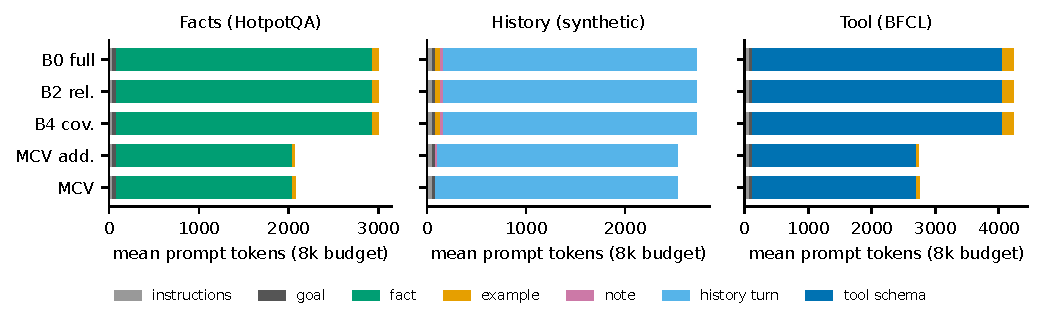
\includegraphics[width= 0.88\linewidth]{../figures/fig5_composition.pdf}
\caption{Mean prompt composition at the 8k budget (test, Qwen3-4B-Instruct). MCV leaves budget unused: it drops the
profile note, most low-value documents and tool schemas, and some worked examples.}\label{fig:composition}
\end{figure}

\subsection{Interactions: H2 Has No Detectable Effect}
Adding interaction terms changed pooled AUBC by \RHTwoPooledDiff{} [\RHTwoPooledLo, \RHTwoPooledHi] (Holm
$p\RHTwoPooledPRel$). History is at ceiling from 2k upward, which leaves little room for any difference, so this null result is limited. The
only large interaction measured is between history and the profile note (\RIntHistoryHistoryTurnNote). Because the note
is current in half of the instances and stale in the other half, the negative sign means the two substitute for each
other: either can supply the answer when it is current, and the note adds nothing once history is present (its own
value is \RMcvHistoryNote). The interaction terms did change the plans: OURS and OURS-A
selected different blocks in \RSelDiffFacts of facts, \RSelDiffHistory of history and \RSelDiffTool of tool plans.
At 8k, OURS never included the note while OURS-A included it in \RHasNoteAdditiveHistory of history plans, and the
positive example--document interaction (\RIntFactsExampleFact) made OURS keep an example in \RHasExampleOursFacts of
facts plans against \RHasExampleAdditiveFacts for OURS-A. These changes concern low-value blocks and rarely changed
success (\RSelOutcomeDiffFacts, \RSelOutcomeDiffHistory and \RSelOutcomeDiffTool of episodes). On these families, type-pair interactions change what is sent but not whether the task succeeds.

\subsection{Post-hoc Follow-up: Stopping Rules and a Hybrid}
The results above leave two questions open: are the token savings specific to MCV, and does the three-level split of
Section~\ref{sec:problem} help if each level uses the signal that worked? After the main results were known we
pre-specified a follow-up (an addendum to the pre-registration, committed before any of its runs) with two policies.
\emph{B2S} is relevance ranking with a stopping rule: blocks whose goal cosine falls below a threshold $\tau$ are never
added. \emph{HYB} is a hybrid: the 4B profile admits only types whose MCV interval excludes zero (documents, history
sessions, tool schemas), relevance ranks blocks within admitted types with value $\cos-\tau$, and the compiler applies the
budget, dependencies and short variants. Each family's $\tau$ was chosen from a five-point grid on \RNCalib development
instances not used for profiling, as the most token-saving value whose success at 8k stayed within \RMargin of full
context. The same rule picked the same $\tau$ for both policies in every family. Both were run on the main test instances
and budgets; H6 tests B2S and H8 tests HYB for non-inferiority to full context at 8k, H7 tests HYB against B2 in AUBC
(one Holm family of nine tests).

\begin{table}[t]\centering\small
\caption{Post-hoc follow-up (test, Qwen3-4B-Instruct, \RNMain instances per family). AUBC; success and prompt-token
reduction relative to full context at 8k. Non-inferiority margin \RMargin.}\label{tab:followup}
\setlength{\tabcolsep}{3pt}
\fitwidth{%
\begin{tabular}{@{}lccc@{}}\toprule
 & Facts & History & Tool\\\midrule
AUBC: B2 / OURS & \RAubcFactsRel{} / \RAubcFactsOurs & \RAubcHistoryRel{} / \RAubcHistoryOurs & \RAubcToolRel{} / \RAubcToolOurs\\
AUBC: B2S / HYB & \RAubcFactsStop{} / \RAubcFactsHyb & \RAubcHistoryStop{} / \RAubcHistoryHyb & \RAubcToolStop{} / \RAubcToolHyb\\
H7: HYB$-$B2 [CI] & \RHSevenFactsDiff{} {\scriptsize[\RHSevenFactsLo, \RHSevenFactsHi]} & \RHSevenHistoryDiff{} {\scriptsize[\RHSevenHistoryLo, \RHSevenHistoryHi]} & \RHSevenToolDiff{} {\scriptsize[\RHSevenToolLo, \RHSevenToolHi]}\\\midrule
@8k success: B0 / OURS & \RSucFullFacts{} / \RSucOursEightFacts & \RSucFullHistory{} / \RSucOursEightHistory & \RSucFullTool{} / \RSucOursEightTool\\
@8k success: B2S / HYB & \RSucFactsStopEight{} / \RSucFactsHybEight & \RSucHistoryStopEight{} / \RSucHistoryHybEight & \RSucToolStopEight{} / \RSucToolHybEight\\
@8k tokens cut: OURS & \RTokCutFacts & \RTokCutHistory & \RTokCutTool\\
@8k tokens cut: B2S / HYB & \RTokCutStopFacts{} / \RTokCutHybFacts & \RTokCutStopHistory{} / \RTokCutHybHistory & \RTokCutStopTool{} / \RTokCutHybTool\\
H6: B2S$-$B0 [CI] & \RHSixFactsDiff{} {\scriptsize[\RHSixFactsLo, \RHSixFactsHi]} & \RHSixHistoryDiff{} {\scriptsize[\RHSixHistoryLo, \RHSixHistoryHi]} & \RHSixToolDiff{} {\scriptsize[\RHSixToolLo, \RHSixToolHi]}\\
\bottomrule\end{tabular}}
\end{table}

Table~\ref{tab:followup} gives the results. \textbf{The hybrid did not improve selection.} HYB exceeded B2 in none of the
three families (H7; Holm-adjusted $p$ \RHSevenFactsP, \RHSevenHistoryP and \RHSevenToolP), and its AUBC was close to that of OURS
(HYB$-$OURS: \RHybVsOursFacts, \RHybVsOursHistory, \RHybVsOursTool). On history its bootstrap interval against B2 lies
entirely below zero (\RHSevenHistoryDiff{} [\RHSevenHistoryLo, \RHSevenHistoryHi]), although the Wilcoxon test is not
significant: its calibrated threshold sometimes excludes the update session itself, at every budget, the same loss
B2S shows on history. \textbf{The type filter added nothing measurable here:} HYB and
B2S produced the same outcome in \RHybStopSame of episodes, although B2S kept an example or the note in most of its plans. This
is consistent with the profiles: the excluded types carry little value, so removing them saves some tokens
(\RTokCutHybTool against \RTokCutStopTool on tool use) without changing outcomes. \textbf{The savings are not specific to MCV.} On tool use,
relevance with a stopping rule was non-inferior to full context at 8k (H6, Holm $p\RHSixToolPRel$) while removing
\RTokCutStopTool of prompt tokens, against \RTokCutTool for OURS; HYB behaved alike (H8, $p\RHEightToolPRel$). On facts and
history the calibrated thresholds were too aggressive for the test set: they removed \RTokCutStopFacts and
\RTokCutStopHistory of tokens, but success fell by \RHSixFactsDiff{} and \RHSixHistoryDiff{}, and non-inferiority was not
shown. There, the more conservative OURS kept success at the cost of smaller savings. A threshold calibrated on
\RNCalib instances is a coarse instrument; the facts calibration curve was not even monotone. On tool use the rule chose the
largest threshold in the grid, so the saving reported there is a lower bound on what a stopping rule could remove.

\subsection{What the Profiles Say}
Fig.~\ref{fig:profiles} and Table~\ref{tab:profiles} show the profiles of both models. Three regularities hold across families. First,
the value of context is concentrated: tool schemas (\RMcvToolToolSchema), documents (\RMcvFactsFact) and history
sessions (\RMcvHistoryHistoryTurn) carry nearly all of it. Second, worked examples are worth close to nothing
on their own (\RMcvFactsExample, \RMcvHistoryExample, \RMcvToolExample on the 4B model; the 8B model valued them
at \RMcvEightHistoryExample on history), although every family's prompt includes them by default. Third, short variants are worth much less than full blocks for tool schemas
(\RShortToolToolSchema against \RMcvToolToolSchema), because the parameter schema matters for argument filling.
The length-neutral control, which replaces a removed type with filler of approximately equal token length (\RPadN instances per
type), reproduced the removal effects: documents \RRemFactsFact by removal against \RPadFactsFact with padding, tool
schemas \RRemToolToolSchema against \RPadToolToolSchema, history \RRemHistoryHistoryTurn against
\RPadHistoryHistoryTurn. The measured values reflect content, not prompt length.


\begin{figure}[t]\centering
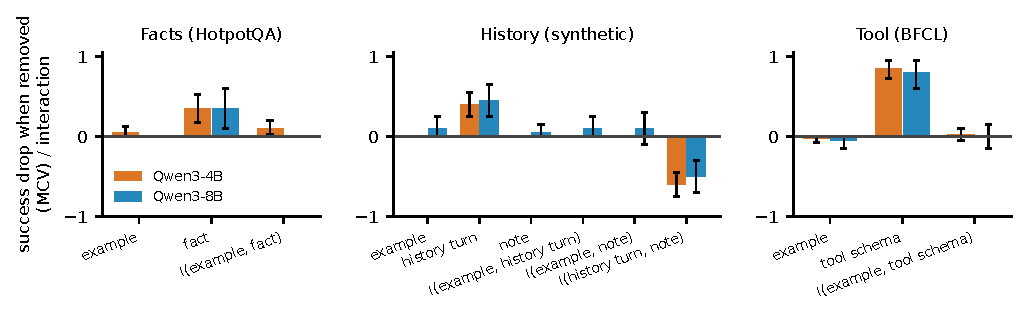
\includegraphics[width= 0.88\linewidth]{../figures/fig3_profiles.pdf}
\caption{MCV profiles (development split): success drop when a type is removed, and pairwise interactions
$I(\tau_1,\tau_2)$, for Qwen3-4B-Instruct (\RNProfFour instances) and Qwen3-8B (\RNProfEight instances), with 95\%
bootstrap CIs.}\label{fig:profiles}
\end{figure}

\subsection{Transfer Across Model Size and Release (H3)}
The 4B and 8B profiles rank the \RRhoN (family, type) values similarly (Spearman $\rho=\RRho$, pooled across families, so
between-family differences contribute to the agreement), and their magnitudes agree
closely (Fig.~\ref{fig:profiles}). On Qwen3-8B (first \RNTransfer test instances per family, budgets 2k and 8k),
compiling with the transferred 4B profile and with the natively measured 8B profile gave a pooled success difference of
\RTransferDiff{} [\RTransferLo, \RTransferHi] over \RTransferN paired episodes, so H3 non-inferiority holds
(Fig.~\ref{fig:transfer}). The outcome was the same in \RTransferAllEqual of paired episodes, giving the degenerate
interval above, although the two profiles
produced identical selections in only \RTransferSameSel. The differences involved tool schemas,
history sessions and examples alike, yet never changed the outcome. This suggests that both profiles keep the blocks
that decide success and differ only in blocks that do not. It equally indicates that, with the block-value model
shared, the compiler's outcomes are insensitive to the type-level profile, so H3 does not show that the profile drives
the decisions that matter. The efficiency pattern of the 4B study carried over. On tool use at 8k the transferred profile
sent \RTrTokToolTransferEight prompt tokens against \RTrTokToolRelEight for relevance ranking, with success
\RTrToolTransferEight against \RTrToolRelEight. Relevance ranking was again more accurate on facts (\RTrFactsRelTwo
against \RTrFactsTransferTwo at 2k). With \RNTransfer instances per family these 8B comparisons are descriptive.


\textbf{Failure analysis.} Transcripts show three failure modes: abstentions when the session holding an update is dropped, identifiers corrupted by LLMLingua-2 compression, and answer changes on facts even when all evidence was kept (Appendix~\ref{app:failures}).

\textbf{Profiling sample size.} In an exploratory subsampling analysis the type-level profile stabilized with ten to twenty development instances per family (Appendix~\ref{app:samplesize}).

\subsection{Cost}
\textbf{Compilation.} Over \RSolves compilations CP-SAT proved optimality in \RSolveOptimal of cases with no fallback
(\RSolveFallback); median solve time was \RSolveMedianMs{} ms (99th percentile \RSolveNinetyNineMs{} ms, maximum
\RSolveMaxMs{} ms), and end-to-end planning including feature computation (with cached block embeddings) took a median \RPlanMedianMs{} ms.
\textbf{Profiling.} The 4B profile cost \RProfCallsTotal model calls (\RProfHours hours on a laptop). Measured in
prompt tokens, profiling pays for itself after about \RBreakEvenTool queries on tool use and \RBreakEvenFacts on
facts, given the 8k-budget savings above. The facts figure is conditional on accepting that family's non-significant success loss. History saves less per query and breaks even after about
\RBreakEvenHistory.



\textbf{Development history.} The block-value model went through three development versions before the method was frozen and pre-registered; all are reported in Appendix~\ref{app:devhistory}.
